%!TEX root = ../../thesis.tex

%=============================================================================


\section{Orchestrator}
\label{main:orc}
In this section the Orchestrator as part of the proposed framework will discussed.
The Orchestrator has to fulfill two major tasks, synchronizing results and determining the formats used to transmit audio, as discussed in the previous chapter \ref{main:lib:format_chooosing}.

\subsubsection{Determining Audio Formats}
First the determination of audio in- \& output formats used internally by the library will be discussed.
To achieve this, a number of factors have to be considered.
To reduce network traffic and improve transmission speed it is advantageous to transmit audio with the lowest possible bandwidth.
Consider two nodes, where one node transmits and one node receives audio which differs only in that one node internally works with 16kHz and the other with 48kHz.
In this scenario, resampling should happen at the node which works with 48kHz, in order to transmit only 16kHz audio.

However, it may be the case that network capacity is abundant while CPU capacity is not, e.g. in embedded systems.
Consider a node outputting an audio signal at 16kHz, and four nodes requiring this audio signal at 48kHz, e.g. a \gls{vad}, gender-, emotion-, and voice recognition.
In this scenario, one may opt to not resample four times, but rather once and transmit the higher bandwidth audio, or, more generally speaking, minimize the number of resamplings happening in the pipeline.

To tackle this issue, I developed two algorithms which could each handle one of these cases and added a simple way to add new algorithms, should the need arise.
The first algorithm introduces a cost function which calculates the bandwidth of each topics formats.
This algorithm is formalized in figure \ref{main:orc:resampling:formula:min_traffic}.
It applies the aforementioned cost function $cost_{format}$ on each in- \& output format for a given topic and then chooses the minimum as the optimal.

\begin{figure}
	\begin{align*}
	cost_{format} &= channel\_count \cdot bitrate_{signal} \cdot frequency\\
	format_{optimal} &= min({bitrate_{i}\ |\ i \in formats_{input} \cup formats_{output}})
	\end{align*}
	\caption{Formula to calculate the lowest bandwidth format out of a given set of in- \& output formats.
		The $bitrate_{signal}$ is the amount of bits a single sample requires, while the $bitrate_{i}$ is the $cost_{format}$ of the format $i$.}
	\label{main:orc:resampling:formula:min_traffic}
\end{figure}

The second algorithm is a bit more complex, as it prioritizes the amount of resamplings over the used bandwidth when choosing the right format.
It is formalized in figure \ref{main:orc:resampling:formula:min_cpu}.
As such, it calculates for each format on a given topic the number of resamplings that would occur, if that format was chosen for this topic.
Then the format which has the fewest resamplings is chosen as the optimal format.
However, there may be several formats which fulfill this condition.
If this is the case, it comes naturally to mind to choose the format which requires the least amount of bandwidth, so the algorithm formalized in figure \ref{main:orc:resampling:formula:min_traffic} is used to choose the optimal format of the formats which require the least amount of resampling.

\begin{figure}
	\begin{align*}
	\alpha(i,k) &=
	\begin{cases}
	1 & , i = k \\
	0 & , i \neq k
	\end{cases} \\[10pt]
	resamplings_{format} &= \sum_{f=1}^{F} \alpha(format, f) ,\ f \in formats\\[10pt]
	format_{optimal} &= argmin_{f}(resamplings_{f}) , \ f \in formats
	\end{align*}
	\caption{Formula to calculate the lowest bandwidth format out of a given set of in- \& output formats.
		The $bitrate_{signal}$ is the amount of bits a single sample requires, while the $bitrate_{format}$ indicates, how many bits a second of this signal require.}
	\label{main:orc:resampling:formula:min_cpu}
\end{figure}

After the Orchestrator determined the transmission format for each topic, it will inform all registered components about their respective internally used audio formats via a \gls{ros}-message.
The library part of each component will listen to these messages and then store and use these formats as discussed in chapter \ref{main:lib:format_chooosing}.
It is important to note at which points in time the Orchestrator will determine the audio formats.
Since it cannot conclusively determine if all components that are going to be started have already registered, as it lacks a list of such components, whenever a component registers the formats of all topics are determined anew.
Additionally, a component may die or shut down at any point in time.
When this is detected, all formats are determined as well, since the Orchestrator cannot foretell how long the pipeline will still run in the current configuration and more profitable audio formats may save a lot of bandwidth or computation time, or improve the quality of the transmission, by not unnecessarily resampling and converting audio.  

Determining whether a component has shut down must be conducted by the Orchestrator.
For this reason it will routinely ping all components via \gls{ros} inbuild \gls{ros}-node pinging functionality.
Should \gls{ros} not find a node in question, or should the node be non-responding, the Orchestrator will remove it from its internally kept list of active nodes and terminate all communication with it.
Such nodes will furthermore not be considered for fusion of results anymore. 

\subsubsection{Result Fusion}

When synchronizing results, a few key circumstances need to be kept in mind.
The first and probably most important one is that because of the library and the relentless efforts to annotate the audio and in turn results with timestamps, the synchronization of the results itself is rather trivial.
There are however still a few possible pitfalls.
Most importantly, the Orchestrator can not know with certainty when results are arriving, or -more precisely- when all of the results to be synchronized will have arrived.
This is rather unfortunate, as it is of utmost importance to relay all information as soon as possible, to keep further programs reliant on the synchronized results, such as natural language processors or robot behavior controllers, not waiting and thus keep latency down to a minimum.
There is another important question, which has been evaded up until now.
When results are synchronized, with respect to what are they synchronized?
After all, results of different types may overlap within the time frame of their respective occurrence.
An example of this phenomenon can be observed in figure \ref{pic:main:orc:result_overlap}.
The first result of an \gls{asr} node, A1, may be fused with the first result of an \gls{ssl} node, S1.
This however occurred partially with A2, which may be also fused for the result.
This could iteratively go on until all shown results may be fused together.
This is naturally not desirable, as the latency of the first results would needlessly increase and no meaningful information could be gained by this synchronization.

\begin{figure}[]
	\centering
	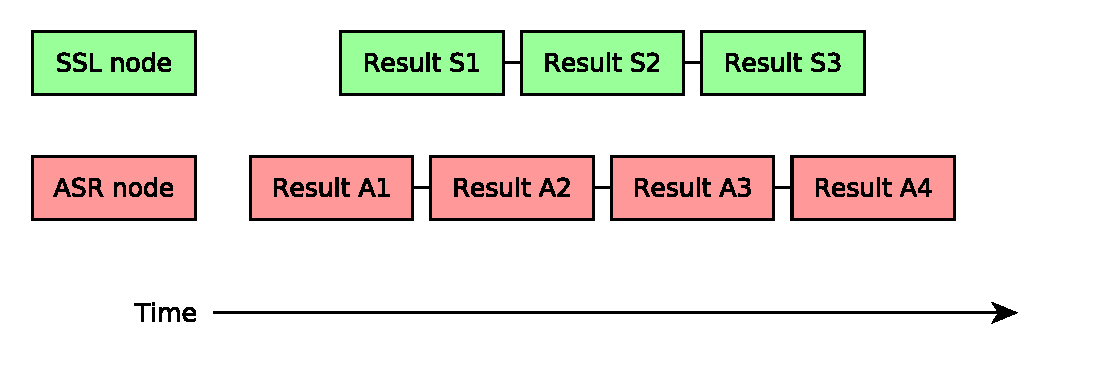
\includegraphics[width=\textwidth]{diagrams/main_orc_result_overlap.pdf}
	\caption{Overlap of results from two distinct components, an \gls{ssl} component in green and an \gls{asr} component in red.
		Trying to synchronize as much results as possible may result in a macro result containing all presented data.}
	\label{pic:main:orc:result_overlap}
\end{figure}


A few approaches to deal with this problem may come to mind.
It could for example be chosen to synchronize with respect to each recorded audio message.
But due to the library not enforcing a singular, constant size for the audio transmitted via these messages (see chapter \ref{main:lib:augmented_audio_msg} and chapter \ref{basics:latency} for the reasoning), this could quickly explode in complexity; especially since a beamformer may create a new artificial audio signal which may either transport smaller audio signals with each message or slightly shift the timestamps of the messages, due to factoring in the time-of-arrival differences for the different microphones.
This way, all -or worse, just some- of the results may have been computed on timestamps differing from the originally recorded ones.

The approach ultimately chosen was to determine one so called anchor type, which would then be the basis of all synchronization.
Each result received of this anchor type would by their timestamps determine the timeframe with which results of all other types would then be synchronized with.
Any result occurring at least partially in this timeframe would be included in the fused result.
This approach is similar to \cite{10.1117/12.138164}, in that my approach also batches results.
Unlike \cite{10.1117/12.138164} however, in my approach batching happens dynamically, based on the anchor result and not on a pre-determined timeframe.

Initially it was planned to only use speech utterances as anchor.
However, as time moved on, I realized that this may not be the only interesting type for synchronization.
Programs for tracking persons for example could be very interested in obtaining data on which particular person was speaking at a given moment, synchronized with their position provided by \gls{ssl} information.
And so the algorithms of the Orchestrator would quickly be adapted to not only use every result type as anchor type, but to do so concurrently.
Thus any result type of particular interest can be provided without giving up synchronization with other results.

In chapter \ref{main:lib}, the fact that each component will register itself giving a designation was discussed.
A list of these designations can be seen in figure \ref{table:main:designations}.
This designation corresponds to a result type, seen on the right side of the figure.
Through this connection the Orchestrator can know to expect certain result types from each component of a pipeline.
A special case in this is the \texttt{Other} designation, which should be assigned to utility components, such as an audio recorder, or a playback node.
The Orchestrator will not expect any results of these components, but still take them into account when determining audio formats.

\begin{figure}[]
	\centering
	\begin{tabular}{| l | r |}
		\hline
		\gls{vad} 		& VADInfo	 	\\ \hline
		SpeechRec		& SpeechInfo		\\ \hline
		\gls{ssl}		& SSLInfo		\\ \hline
		Gender			& GenderInfo		\\ \hline
		Emotion			& EmotionInfo		\\ \hline
		VoiceId			& VoiceIdInfo		\\ \hline
		Other 			& None	 	\\ \hline
	\end{tabular}
	\caption{Possible designations of components along with result messages (see figure \ref{table:main:lib:messages}) expected from them.}
	\label{table:main:designations}
\end{figure}

The Orchestrator may receive results in any order.
However, fused results should not be published, until all results of interest were received.
When the Orchestrator receives a result of one of his anchor types, results of interest may already have been received, or still be to be received.
Thus a way to gather all these results is needed.
To take care of all results the Orchestrator has already received, it was chosen to create a database, in which all incoming results are saved.
This may seem a little over-engineered, but will later be of additional service.

When the Orchestrator receives a result of its anchor type, it will then create a so called \texttt{Fusion} object.
This object will store all relevant results and additional information used to fuse the results.
It starts by querying the database for all results which occurred in the timeframe predefined by the anchor result.
If will then continue to collect incoming results, if they are eligible for fusion until it determines that no new results will be received.

\subsubsection{Fusion Conditions}
This can happen in either of two ways.
The first, straight forward way is the case if all possible results are already present.
As the timestamps of the audio is continuous, the results can be as well.
Such is the case in figure \ref{pic:main:orc:all_results}, where the results produced by the \gls{ssl} component are continuous and do not allow for another result of the same type to occur.
If this is detected, the results may be fused an published as an synchronized result immediately.

\begin{figure}[]
	\centering
	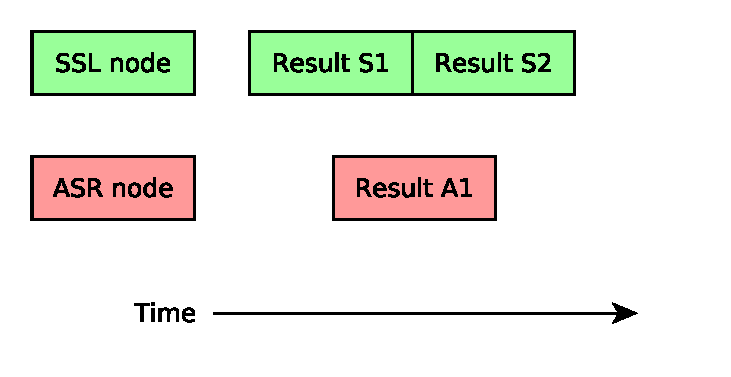
\includegraphics[width=.66\textwidth]{diagrams/main_orc_all_results.pdf}
	\caption{Complete overlap of results.
		If the \gls{asr} component publishes the anchor type, and these need only be synchronized with \gls{ssl} results, it can be determined that all relevant information was gathered as soon as \textit{Result S2} was received.}
	\label{pic:main:orc:all_results}
\end{figure}

The second to determine if no more results will be received is more complex.
Components should not be expected to produce results for every bit of sound they receive.
More explicitly, components should be expected to sometimes not produce results, e.g. if they are unsure of their result or if they could not detect something.
As an example, consider an \gls{ssl} component to produce a result based on a shattering glass.
Other components, especially components requiring an actual utterance or at least a voice to be present in the signal should not detect anything during this time and thus not produce any results.
This would make synchronizing the generated \gls{ssl} results with anything other impossible. 
Additionally, it must be kept in mind that components may unexpectedly shut down.
Synchronizing their then not produced results would be impossible.
A component may also struggle to calculate one specific result, due to it being either very computationally expensive or due to having a temporary shortage of computational power, because e.g. other programs consuming much computational power.

\subsubsection{Fusion Timeouts}
To counter this problem a timeout is needed that will tell the Orchestrator to abandon any results not yet received.
This is somewhat contrary to the previously discussed goal of ensuring the synchronization of all results, but is crucial to ensure all results to be actually relayed to further programs and arrive there with a minimal latency.
Finding a feasible value for this timeout is not trivial, as circumstances can have a major impact on it.
Consider for example a setup running over a slow, but very stable network connection, or a number of components running on very weak hardware.
In both cases the timeout should be bigger than normal.

An optimal timeout may also be dependent on the components used in a specific pipeline configuration.
Consider a setup with a component which is very fast in computing results and one which takes a long time for this.
In the case the fast component did not produce a result, a long timeout would lead to a higher latency than a small one.
A large timeout would however be needed for the component which takes a long time to produce results.

\label{main:orc:database}
The method I developed to find the optimal timeout takes into account all of these concerns.
Making use of the database included to save results, not only received results are saved, but also their time to compute.
This can very easily be calculated, as this is just the difference between the time the result is received by the Orchestrator and the end time of the audio timestamp.
This gives the absolute time needed from recording the audio to the point in time at which results are available to the Orchestrator.
Because this time is generated for each result, the average for each type of result can then be calculated.
Thus a timeout for each type of result can be generated, which is equivalent to a timeout for each component.
To avoid ignoring results which take shortly longer to arrive at the Orchestrator than the average, the average value is multiplied with a constant factor to gain the final timeout.
I found a factor of 1.5 to work quite well in this regards.

These timeouts are generated for each anchor result anew.
Due to this, the Orchestrator can react to possible changes in the execution times of components and adjust the timestamps on the fly.
The first anchor result the Orchestrator receives however will not be able to generate timeouts this way, an alternative is needed for it.
I found a hard coded high timeout and the thusly potentially higher latency resulting on this first result to be acceptable.
However, at this point another feature of the database approach from before comes in.
As results are stored permanently, it is possible to simply load an already existing database.
If the configuration of the used pipelines have not changed to much with respect to components and network/ compute environment, the Orchestrator can make use of the previous runs and thus eliminate the drawback of the first anchor result.

%-------------------------

\subsubsection{Latency caused by Fusion}
Lastly the latency introduced by synchronizing results is worth a look at.
In a best case scenario, where the Orchestrator can make use of overlapping results (as shown in figure \ref{pic:main:orc:result_overlap}), the latency is simply the time of the slowest computing component, along with a small calculation time the Orchestrator introduces.
The worst case scenario can be seen in figure \ref{main:orc:latency:formula}.
This latency $l_f$ is mostly determined by the exact factors discussed previously: The maximum of the average time to compute of all components and the multiplicand $V_A$. 
I consider this to be a worthwhile trade off, due to the most important anchor message types only being generated when an utterance or at least voice is present in the corresponding audio.
I believe these message types to be that of the \gls{asr}-, emotion-, gender-, and voice-results.

\begin{figure}
	\begin{align*}
	l_{f} = V_A \cdot max(\{\frac{1}{n_i} \cdot \sum_{k=1}^{n_i} l_{i,k}\ | \ i \in components\})
	\end{align*}
	\caption{Maximum latency of a single fusion.
		$V_A$ is a constant.
		$n_i$ is the amount of results the orchestrator already received of a component $i$.
		$l_{i,k}$ is the latency of the $k$th result of the component $i$.}
	\label{main:orc:latency:formula}
\end{figure}
